% ********** Rozdział 4 **********
\chapter{Harmonogram realizacji projektu}
Realizacja projektu "Zarządzanie pojazdami" została zaplanowana i przeprowadzona zgodnie z harmonogram realizacji projektu oparrtym na diagram Gantta. Przedstawia on poszczególne etapy projektu rozłożone w czasie.


\begin{figure}[h] 
    \centering
    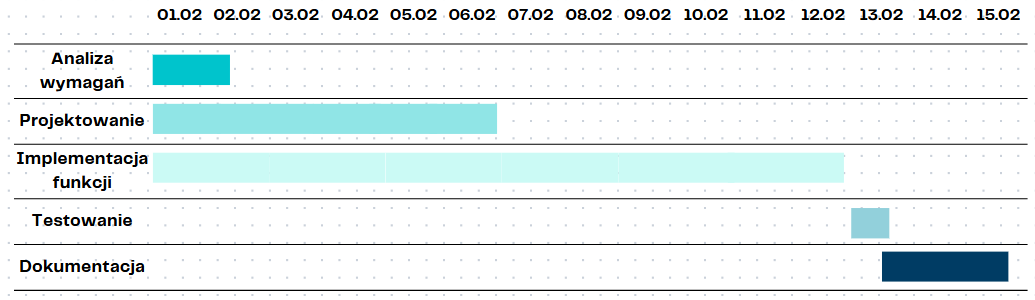
\includegraphics[width=1\textwidth]{Daigram gaunt.png}
    \caption{Diagram Gauntta}
    \label{fig:moj_obrazek}
\end{figure}
Etapy realizacji projektu na podstawie diagramu Gantta:
\begin{itemize}
    \item Analiza wymagań – określenie funkcjonalności i wymagań projektu.
    \item Projektowanie systemu – zaprojektowanie struktury klas, interfejsów i diagramu klas.
    \item Implementacja systemu – implementacja klas, interfejsów i testowanie funkcjonalności.
    \item Testowanie systemu – sprawdzenie poprawności działania systemu i naprawa błędów.
    \item Dokumentacja projektu – przygotowanie dokumentacji technicznej i użytkownika.
\end{itemize}
\section*{Repozytoriun i system kontroli wersji}
Projekt został zrealizowany z wykorzystaniem systemu kontroli wersji Git oraz platformy GitHub. Repozytorium projektu znajduje się pod adresem: \url{https://github.com/w69760/Labolatoria}
% ********** Koniec rozdziału **********